\chapter{Implementation}
\label{ch:implementation}

This chapter describes how the design of \cref{ch:design} was realized in
code. The application, internally named \texttt{offline\_first}, is
implemented as a single Kotlin Multiplatform Gradle module,
\texttt{composeApp}, targeting Android (API 24+) and iOS (via a static
Kotlin/Native framework consumed by a thin SwiftUI host app). All code
excerpts in this chapter are taken, with minor trimming for length, from
the actual project source tree.

\section{Toolchain and Dependencies}
\label{sec:toolchain}

\Cref{tab:toolchain} lists the core technologies used, managed through a
Gradle version catalog (\texttt{libs.versions.toml}) shared by the module.

\begin{table}[htbp]
\centering
\caption{Core toolchain and libraries.}
\label{tab:toolchain}
\begin{tabularx}{\textwidth}{@{}l X@{}}
\toprule
\textbf{Concern} & \textbf{Library / tool} \\
\midrule
Language \& multiplatform & Kotlin, Kotlin Multiplatform Gradle plugin \\
UI & Compose Multiplatform (Material 3), Navigation-Compose \\
Local persistence & AndroidX Room (multiplatform artifact) over the
bundled cross-platform SQLite driver (\texttt{androidx.sqlite:sqlite-\allowbreak
bundled}), with Room's KSP compiler generating DAO implementations for
Android, iOS x64, iOS Arm64, and iOS Simulator Arm64 \\
Backend SDK & GitLive \texttt{firebase-kotlin-sdk} (\texttt{firebase-common},
\texttt{firebase-firestore}, \texttt{firebase-auth}) -- a Kotlin
Multiplatform wrapper over the native Firebase Android and iOS SDKs \\
Concurrency & Kotlin Coroutines (\texttt{kotlinx-coroutines-core}),
\texttt{kotlinx-datetime}, \texttt{kotlin.time.Clock} \\
Serialization & \texttt{kotlinx-serialization-json} \\
Local key-value storage & \texttt{multiplatform-settings} (session flags) \\
Cryptography & \texttt{org.kotlincrypto} (HMAC-SHA256, secure random) for
local password hashing \\
Image loading & Coil (\texttt{coil-compose}), multiplatform \\
Android-only & AndroidX Credentials API + Google ID (Google Sign-In) \\
\bottomrule
\end{tabularx}
\end{table}

A defining implementation choice, already introduced in
\cref{sec:local-storage-design}, is the use of \textbf{Room in Kotlin
Multiplatform mode}. \Cref{lst:database} shows the actual database
declaration. Because Kotlin/Native cannot use JVM reflection, Room's KSP
processor generates a per-target \texttt{actual object
AppDatabaseConstructor} that instantiates the generated implementation
directly (line 29); this is the one piece of Room "magic" that requires a
platform-specific counterpart, and it is entirely generated code -- no
project code touches it.

\begin{lstlisting}[language=Kotlin, caption={Room database declaration (\texttt{data/local/AppDatabase.kt}).}, label={lst:database}]
const val DATABASE_NAME = "offline_first.db"

@Database(entities = [Report::class, User::class], version = 6, exportSchema = false)
@TypeConverters(Converters::class)
@ConstructedBy(AppDatabaseConstructor::class)
abstract class AppDatabase : RoomDatabase() {
    abstract fun reportDao(): ReportDao
    abstract fun userDao(): UserDao
}

@Suppress("NO_ACTUAL_FOR_EXPECT")
expect object AppDatabaseConstructor : RoomDatabaseConstructor<AppDatabase> {
    override fun initialize(): AppDatabase
}

fun RoomDatabase.Builder<AppDatabase>.buildAppDatabase(): AppDatabase =
    fallbackToDestructiveMigration(dropAllTables = true)
        .setDriver(BundledSQLiteDriver())
        .setQueryCoroutineContext(ioDispatcher)
        .build()
\end{lstlisting}

\section{Local Persistence Layer}
\label{sec:impl-persistence}

The \texttt{Report} entity (\cref{lst:report-entity}) is the direct
implementation of the schema designed in \cref{fig:er-diagram}: a Room
\texttt{@Entity} whose fields are exactly the columns of
\cref{tab:report-fields}, with \texttt{syncStatus} typed as the
\texttt{SyncStatus} enum from \cref{fig:sync-state-machine} rather than a
raw string, so that the compiler -- not a runtime check -- rejects any
attempt to write an undefined status.

\begin{lstlisting}[language=Kotlin, caption={The \texttt{Report} entity (\texttt{data/model/Report.kt}).}, label={lst:report-entity}]
@Entity(tableName = "reports")
data class Report(
    @PrimaryKey(autoGenerate = true)
    val id: Long = 0,

    val localId: String,       // UUID, generated on creation
    val remoteId: String?,     // Firestore document ID, null until synced

    val title: String,
    val description: String,
    val category: String,
    val location: String,
    val photoPath: String?,
    val remotePhotoUrl: String? = null,

    val owner: String,         // email of the user who created the report
    val createdAt: Long,
    val updatedAt: Long,

    val syncStatus: SyncStatus
)
\end{lstlisting}

The category values actually shipped
(\texttt{REPORT\_CATEGORIES} in \texttt{AddReportViewModel}, listed in
\cref{tab:toolchain}'s surrounding code) are a general-purpose civic-issue
taxonomy -- \emph{Infrastructure, Public Safety, Vandalism, Sanitation,
Environment, Other} -- rather than a literal enumeration of the five
example reports from \cref{sec:case-study} (broken projector, damaged
chair, Wi-Fi issue, AC problem, missing lab equipment). This is an
intentional generalization: those five examples map naturally onto
\emph{Infrastructure} (projector, chair, AC, lab equipment) and
\emph{Public Safety}/\emph{Other}, and the broader taxonomy keeps the app
usable for the full range of campus facility issues rather than only the
five illustrative examples from the brief.

\Cref{lst:reportdao} shows \texttt{ReportDao}, the sole gateway to the
\texttt{reports} table. Two methods deserve attention:
\texttt{getByOwnerFlow} returns a \texttt{Flow}, so Room re-runs the query
and emits a new list every time any row in \texttt{reports} changes --
this is the mechanism, not any explicit "refresh" call, that makes the
report list update itself the moment a background sync flips a row from
\texttt{PENDING} to \texttt{SYNCED} (\cref{sec:impl-sync}). \texttt{getPending}
and \texttt{getDeletedPending} are the two queries that define the
synchronization module's work queues, directly implementing the "one table,
filtered by status" design decision of \cref{sec:local-storage-design}.

\begin{lstlisting}[language=Kotlin, caption={\texttt{ReportDao} (\texttt{data/local/ReportDao.kt}).}, label={lst:reportdao}]
@Dao
interface ReportDao {
    @Insert(onConflict = OnConflictStrategy.REPLACE)
    suspend fun insert(report: Report): Long

    @Update
    suspend fun update(report: Report)

    @Delete
    suspend fun delete(report: Report)

    @Query("SELECT * FROM reports WHERE owner = :owner ORDER BY createdAt DESC")
    fun getByOwnerFlow(owner: String): Flow<List<Report>>

    @Query("SELECT * FROM reports WHERE id = :id LIMIT 1")
    fun getByIdFlow(id: Long): Flow<Report?>

    @Query("SELECT * FROM reports WHERE syncStatus = 'PENDING'")
    suspend fun getPending(): List<Report>

    @Query("SELECT * FROM reports WHERE syncStatus = 'DELETED_PENDING'")
    suspend fun getDeletedPending(): List<Report>
}
\end{lstlisting}

\section{Authentication and Offline Sessions}
\label{sec:impl-auth}

OFR-2 (offline session continuity, \cref{sec:offline-req}) required more
than simply caching Firebase's own session token, because Firebase
Authentication's SDK itself needs network access for some operations and
because the requirement is specifically that a user can reach the
authenticated part of the app \emph{without} depending on a live
Firebase round trip. The implementation therefore layers a second,
fully local authentication path underneath Firebase Auth: a \texttt{User}
row (email, salted password hash) stored in Room, checked by
\texttt{MainViewModel.checkSession} (\cref{lst:checksession}) whenever
\texttt{Firebase.auth.currentUser} is unavailable but a locally-cached
session (\texttt{SessionStore}, backed by \texttt{multiplatform-settings})
indicates a recent login.

\begin{lstlisting}[language=Kotlin, caption={Session resolution, preferring the live Firebase session but falling back to the local one (\texttt{viewmodel/MainViewModel.kt}).}, label={lst:checksession}]
suspend fun checkSession(): SessionResult {
    val loginTime = sessionStore.loginTimeMillis
    val elapsed = Clock.System.now().toEpochMilliseconds() - loginTime

    if (loginTime > 0L && elapsed > SessionStore.SESSION_DURATION_MS) {
        auth.signOut()
        sessionStore.clear()
        return SessionResult.SessionExpired
    }

    val firebaseUser: FirebaseUser? = auth.currentUser
    if (firebaseUser != null) {
        return SessionResult.LoggedIn(firebaseUser.displayName.orEmpty(), firebaseUser.email.orEmpty())
    }

    val localEmail = sessionStore.localAuthEmail
    if (localEmail != null && loginTime > 0L) {
        val localUser = userDao.findByEmail(localEmail)
        return SessionResult.LoggedIn(localUser?.displayName.orEmpty(), localEmail)
    }

    return SessionResult.NotLoggedIn
}
\end{lstlisting}

The local password hash is computed with PBKDF2-HMAC-SHA256 (100{,}000
iterations, 256-bit derived key, 16-byte random salt), implemented from
multiplatform primitives (\texttt{org.kotlincrypto}) rather than
\texttt{javax.crypto}, so the exact same algorithm runs on Android and iOS
and a hash produced on one platform verifies correctly on the other --
relevant because the underlying \texttt{User} row is a normal Room entity
and could, in principle, itself be part of a future sync path
(\cref{sec:future-work}). A constant-time comparison
(\texttt{constantTimeEquals}) is used when verifying a hash to avoid
leaking timing information about how many leading bytes matched.

\section{Connectivity Monitoring}
\label{sec:impl-connectivity}

The \texttt{ConnectivityObserver} \texttt{expect}/\texttt{actual} pair
(designed in \cref{sec:connectivity-design}) is implemented natively on
each platform. \Cref{lst:connectivity-android,lst:connectivity-ios} show
both implementations side by side; despite using completely different OS
APIs, they present an identical contract to the rest of the app
(\texttt{Flow<Boolean>}, current state emitted immediately, subsequent
changes deduplicated via \texttt{distinctUntilChanged}).

\begin{lstlisting}[language=Kotlin, caption={Android implementation, wrapping \texttt{ConnectivityManager.NetworkCallback} (\texttt{sync/ConnectivityObserver.android.kt}).}, label={lst:connectivity-android}]
class AndroidConnectivityObserver(private val context: Context) : ConnectivityObserver {
    private val cm = context.getSystemService(Context.CONNECTIVITY_SERVICE) as ConnectivityManager

    override val isOnline: Flow<Boolean> = callbackFlow {
        val callback = object : ConnectivityManager.NetworkCallback() {
            override fun onAvailable(network: Network) { trySend(true) }
            override fun onLost(network: Network) { trySend(false) }
            override fun onCapabilitiesChanged(network: Network, caps: NetworkCapabilities) {
                val validated = caps.hasCapability(NetworkCapabilities.NET_CAPABILITY_INTERNET)
                        && caps.hasCapability(NetworkCapabilities.NET_CAPABILITY_VALIDATED)
                trySend(validated)
            }
        }
        val request = NetworkRequest.Builder()
            .addCapability(NetworkCapabilities.NET_CAPABILITY_INTERNET)
            .build()
        cm.registerNetworkCallback(request, callback)
        trySend(isOnline(context)) // emit current state immediately
        awaitClose { cm.unregisterNetworkCallback(callback) }
    }.distinctUntilChanged()
}
\end{lstlisting}

\begin{lstlisting}[language=Kotlin, caption={iOS implementation, wrapping \texttt{NWPathMonitor} via Kotlin/Native cinterop (\texttt{sync/ConnectivityObserver.ios.kt}).}, label={lst:connectivity-ios}]
class IosConnectivityObserver : ConnectivityObserver {
    override val isOnline: Flow<Boolean> = callbackFlow {
        val monitor = nw_path_monitor_create()
        val queue = dispatch_queue_create("offline_first.connectivity.observer", null)
        nw_path_monitor_set_queue(monitor, queue)
        nw_path_monitor_set_update_handler(monitor) { path ->
            trySend(nw_path_get_status(path) == nw_path_status_satisfied)
        }
        nw_path_monitor_start(monitor)
        awaitClose { nw_path_monitor_cancel(monitor) }
    }.distinctUntilChanged()
}
\end{lstlisting}

Both callback-based OS APIs are adapted into a coroutine \texttt{Flow}
using \texttt{callbackFlow}, which is the standard bridge between
callback-style platform APIs and Kotlin's structured concurrency; note
that \texttt{ConnectivityObserver} itself, and every consumer of it, is
100\% common code. Connectivity monitoring is the only feature in the
whole synchronization path that needed a native implementation at all, and
even there the amount of platform-specific code is small (17 and 15
non-blank lines respectively).

\section{Synchronization Module}
\label{sec:impl-sync}

\texttt{SyncManager} (\cref{lst:syncmanager}) is the direct implementation
of the algorithm designed in \cref{sec:sync-algorithm}: it reads the
pending queue from \texttt{ReportDao}, pushes each report to Firestore
using \texttt{set()} against a document keyed by \texttt{remoteId} if
already known, or by \texttt{localId} otherwise, and updates the local row
to \texttt{SYNCED} on success -- leaving it untouched (implicitly
\texttt{PENDING}, or explicitly demoted to \texttt{FAILED} in a fuller
error-handling pass) on failure. Deletions pending remote confirmation are
processed by a second pass, \texttt{deleteRemotePending}.

\begin{lstlisting}[language=Kotlin, caption={\texttt{SyncManager} (\texttt{sync/SyncManager.kt}), the module implementing \cref{alg:sync}.}, label={lst:syncmanager}]
class SyncManager(private val dao: ReportDao) {
    private val collection = Firebase.firestore.collection("reports")

    suspend fun sync(): Int {
        val pending = dao.getPending()
        val uploaded = uploadPending(pending)
        deleteRemotePending()
        return uploaded
    }

    private suspend fun uploadPending(pending: List<Report>): Int {
        var count = 0
        for (report in pending) {
            try {
                val docRef = if (report.remoteId != null)
                    collection.document(report.remoteId)
                else
                    collection.document(report.localId)

                docRef.set(report.toRemote())
                dao.update(report.copy(
                    remoteId = docRef.id,
                    syncStatus = SyncStatus.SYNCED,
                    updatedAt = Clock.System.now().toEpochMilliseconds()
                ))
                count++
            } catch (e: Exception) {
                // report stays PENDING; next sync trigger will retry it
                println("SyncManager: upload FAILED for ${report.localId}: ${e.message}")
            }
        }
        return count
    }

    private suspend fun deleteRemotePending() {
        for (report in dao.getDeletedPending()) {
            try {
                collection.document(report.remoteId ?: report.localId).delete()
                dao.delete(report)
            } catch (e: Exception) {
                println("SyncManager: delete FAILED for ${report.localId}: ${e.message}")
            }
        }
    }
}
\end{lstlisting}

Two observations connect this listing back to the design decisions of
\cref{sec:sync-design}. First, using \texttt{report.localId} as the
fallback document ID (line 10 of \cref{lst:syncmanager}) is exactly the
idempotency mechanism of \cref{alg:sync}: calling \texttt{sync()} twice in
a row on the same pending report calls \texttt{set()} on the same document
both times, so no duplicate is created even if the first call's local
\texttt{dao.update} did not get a chance to run (e.g. process death
between the network call succeeding and the local write). Second, the
current \texttt{uploadPending} function only ever \emph{writes} to
Firestore -- there is no corresponding read-and-compare of the remote
document's own \texttt{updatedAt} before overwriting it. This is precisely
the "push-only" gap flagged in \cref{sec:conflict-design}: the code as
written always lets the most recent local push win, which is a strict
subset of the bidirectional last-write-wins policy that OFR-7 specifies.
\Cref{sec:conflict-eval} evaluates the practical effect of this gap, and
\cref{sec:future-work} scopes the fix (fetch-then-compare before
\texttt{set()}, or a Firestore transaction).

\subsection{Wiring: connectivity-triggered auto-sync}

\Cref{lst:autosync} shows how \texttt{SyncManager} and
\texttt{ConnectivityObserver} are wired together, inside
\texttt{MainViewModel.loadHome}, to implement OFR-5 and the first trigger
of \cref{sec:sync-triggers}. This four-line \texttt{collect} block is, in
the original codebase's own description, "the single most important
behavior in this app": every other synchronization trigger (cold start,
manual retry, \cref{lst:syncnow}) is a variation on calling
\texttt{syncManager.sync()}, but this is the one that requires \emph{no}
user action at all.

\begin{lstlisting}[language=Kotlin, caption={Auto-sync subscription, started once per login (\texttt{viewmodel/MainViewModel.kt}).}, label={lst:autosync}]
syncJob = viewModelScope.launch {
    connectivityObserver.isOnline.collect { online ->
        if (online) {
            withContext(ioDispatcher) { syncManager.sync() }
        }
    }
}
\end{lstlisting}

Because \texttt{getByOwnerFlow} (\cref{lst:reportdao}) is collected by the
same ViewModel in a sibling coroutine, the report list on screen updates
itself automatically the moment this block's call to \texttt{sync()}
writes new \texttt{SYNCED} statuses to Room -- no manual "refresh the UI"
step is needed anywhere in the sync path, which is the practical payoff of
the reactive, \texttt{Flow}-based architecture chosen in
\cref{sec:mobile-architecture}.

Manual synchronization (FR-9) is exposed as a suspend function,
\texttt{syncNow} (\cref{lst:syncnow}), used by a pull-to-refresh gesture
and by a retry action on failed reports; it distinguishes three outcomes
(nothing to do, offline, synced $n$ reports) so the UI can show an
appropriate message rather than a generic spinner.

\begin{lstlisting}[language=Kotlin, caption={Manual sync entry point (\texttt{viewmodel/MainViewModel.kt}).}, label={lst:syncnow}]
suspend fun syncNow(): SyncOutcome {
    val hasPending = withContext(ioDispatcher) {
        dao.getPending().isNotEmpty() || dao.getDeletedPending().isNotEmpty()
    }
    return when {
        !hasPending -> SyncOutcome.UpToDate
        !isNetworkOnline() -> SyncOutcome.Offline
        else -> SyncOutcome.Synced(withContext(ioDispatcher) { syncManager.sync() })
    }
}
\end{lstlisting}

\section{Report Creation Flow}
\label{sec:impl-create}

\texttt{AddReportViewModel.submitReport} (\cref{lst:submitreport})
implements FR-2/FR-3/OFR-1/OFR-3 directly: validation happens purely
in-memory, and on success the function performs exactly one operation --
an insert into Room -- with a \texttt{localId} generated client-side via
Kotlin's \texttt{Uuid.random()} and an initial \texttt{syncStatus} of
\texttt{PENDING}. No network call appears anywhere in this function; the
report is, from the user's point of view, saved the instant Room's insert
returns, typically within a few milliseconds.

\begin{lstlisting}[language=Kotlin, caption={Report creation (excerpt of \texttt{viewmodel/AddReportViewModel.kt}).}, label={lst:submitreport}]
val now = Clock.System.now().toEpochMilliseconds()
val owner = auth.currentUser?.email.orEmpty()
val report = Report(
    localId = Uuid.random().toString(),
    remoteId = null,
    title = title,
    description = description,
    category = category,
    location = location,
    photoPath = state.photoPath,
    owner = owner,
    createdAt = now,
    updatedAt = now,
    syncStatus = SyncStatus.PENDING
)
viewModelScope.launch {
    withContext(ioDispatcher) { dao.insert(report) }
    _events.value = AddReportEvent.Saved("Report saved locally.")
}
\end{lstlisting}

Editing an existing report (also handled by
\texttt{AddReportViewModel.submitReport}) follows the same pattern but
demotes the report back to \texttt{PENDING} regardless of its previous
status and refreshes \texttt{updatedAt}, so that (a) an edited, previously
\texttt{SYNCED} report is picked up by the next sync pass, and (b) the new
\texttt{updatedAt} is the timestamp the last-write-wins policy
(\cref{sec:conflict-design}) will compare against.

\section{User Interface}
\label{sec:impl-ui}

The UI layer consists of five Compose Multiplatform screens
(\cref{tab:screens}), composed via \texttt{Navigation-Compose} in a single
\texttt{NavHost} (\cref{lst:navhost}) that is itself common code -- the
Android and iOS entry points (\texttt{MainActivity} and
\texttt{MainViewController} respectively) differ only in how they create
the platform \texttt{AppContainer} and supply platform actions (photo
capture, Google Sign-In) that Compose cannot express directly.

\begin{table}[htbp]
\centering
\caption{Screens of the CampusFix mobile client.}
\label{tab:screens}
\begin{tabularx}{\textwidth}{@{}l X@{}}
\toprule
\textbf{Screen} & \textbf{Purpose} \\
\midrule
\texttt{LoginScreen} & Email/password login (Firebase Auth, with local
fallback per \cref{sec:impl-auth}) and Google Sign-In entry point. \\
\texttt{SignUpScreen} & Account creation. \\
\texttt{ReportListScreen} & Primary "home" screen: reactive list of the
user's reports, each annotated with a colored sync-status chip
(\cref{lst:syncstatusui}); pull-to-refresh triggers \texttt{syncNow}. \\
\texttt{AddReportScreen} & Create/edit form (title, category, description,
location, photo); reused for both flows via an optional
\texttt{editingReportId}. \\
\texttt{ReportDetailScreen} & Full detail of a single report, including
its sync status and created/updated timestamps; entry point to edit or
delete. \\
\bottomrule
\end{tabularx}
\end{table}

\begin{lstlisting}[language=Kotlin, caption={Navigation graph (excerpt of \texttt{ui/App.kt}).}, label={lst:navhost}]
NavHost(navController = navController, startDestination = Routes.HOME) {
    composable(Routes.LOGIN) { /* LoginScreen */ }
    composable(Routes.SIGNUP) { /* SignUpScreen */ }
    composable(Routes.HOME) {
        val viewModel = viewModel(key = "main") { MainViewModel(container) }
        ReportListScreen(
            viewModel = viewModel,
            onOpenReport = { id -> navController.navigate(Routes.reportDetail(id)) },
            onAddReport = { navController.navigate(Routes.ADD_REPORT) },
            /* ... */
        )
    }
    composable(Routes.ADD_REPORT) { /* AddReportScreen, create mode */ }
    composable(Routes.EDIT_REPORT, arguments = listOf(navArgument(Routes.ARG_REPORT_ID) { type = NavType.LongType })) {
        /* AddReportScreen, edit mode */
    }
    composable(Routes.REPORT_DETAIL, arguments = listOf(navArgument(Routes.ARG_REPORT_ID) { type = NavType.LongType })) {
        /* ReportDetailScreen */
    }
}
\end{lstlisting}

Sync-state visibility (NFR-5) is implemented as a small pure function,
\texttt{syncStatusInfo} (\cref{lst:syncstatusui}), mapping each
\texttt{SyncStatus} value to a label, color, and Material icon, used by
both the report list item and the report detail screen so the same visual
language (green cloud = synced, orange upload icon = pending, red = failed
or delete-pending) appears everywhere a report is shown.

\begin{lstlisting}[language=Kotlin, caption={Sync status to UI mapping (\texttt{ui/util/SyncStatusUi.kt}).}, label={lst:syncstatusui}]
data class SyncStatusInfo(val label: String, val color: Color, val icon: ImageVector)

fun syncStatusInfo(status: SyncStatus): SyncStatusInfo = when (status) {
    SyncStatus.SYNCED -> SyncStatusInfo("Synced", SyncSynced, Icons.Default.CloudDone)
    SyncStatus.PENDING -> SyncStatusInfo("Pending", SyncPending, Icons.Default.CloudUpload)
    SyncStatus.FAILED -> SyncStatusInfo("Failed", SyncDeleting, Icons.Default.CloudOff)
    SyncStatus.DELETED_PENDING -> SyncStatusInfo("Delete Pending", SyncDeleting, Icons.Default.Restore)
}
\end{lstlisting}

\Cref{fig:screens-wireframe} sketches the report list and add-report
screens at a wireframe level, to give a visual sense of where sync status
is surfaced; these are schematic mockups of the actual Compose layouts,
not screenshots.

\begin{figure}[htbp]
  \centering
  \begin{subfigure}[t]{0.47\textwidth}
    \centering
    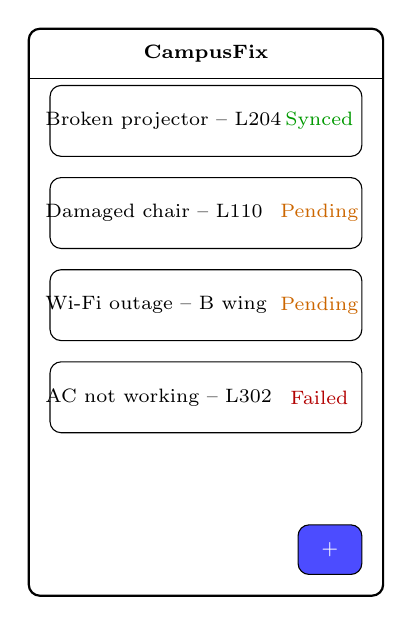
\begin{tikzpicture}[scale=0.9, every node/.style={font=\scriptsize}]
      \draw[rounded corners, thick] (0,0) rectangle (5,8);
      \draw (0,7.3) -- (5,7.3);
      \node at (2.5,7.65) {\bfseries CampusFix};
      \foreach \y/\lbl/\col/\stat in {
        6.2/Broken projector -- L204/green!60!black/Synced,
        4.9/Damaged chair -- L110/orange!80!black/Pending,
        3.6/Wi-Fi outage -- B wing/orange!80!black/Pending,
        2.3/AC not working -- L302/red!70!black/Failed} {
        \draw[rounded corners] (0.3,\y) rectangle (4.7,\y+1);
        \node[align=left, text width=3.0cm] at (1.9,\y+0.5) {\lbl};
        \node[\col] at (4.1,\y+0.5) {\stat};
      }
      \draw[fill=blue!70, rounded corners] (3.8,0.3) rectangle (4.7,1.0);
      \node[white] at (4.25,0.65) {+};
    \end{tikzpicture}
    \caption{Report list: every row shows a sync-status label.}
  \end{subfigure}
  \hfill
  \begin{subfigure}[t]{0.47\textwidth}
    \centering
    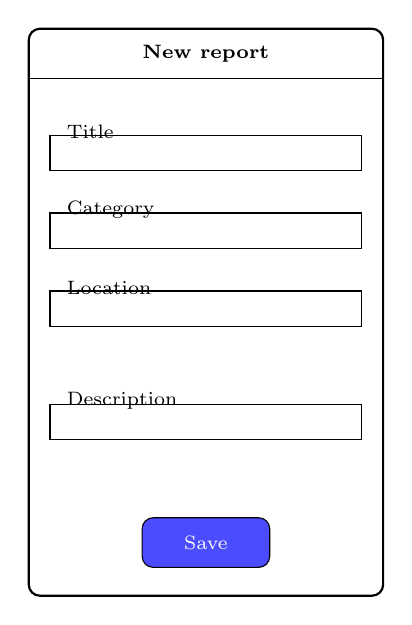
\begin{tikzpicture}[scale=0.9, every node/.style={font=\scriptsize}]
      \draw[rounded corners, thick] (0,0) rectangle (5,8);
      \draw (0,7.3) -- (5,7.3);
      \node at (2.5,7.65) {\bfseries New report};
      \foreach \y/\lbl in {6.0/Title, 4.9/Category, 3.8/Location, 2.2/Description} {
        \node[anchor=west] at (0.4,\y+0.55) {\lbl};
        \draw (0.3,\y) rectangle (4.7,\y+0.5);
      }
      \draw[fill=blue!70, rounded corners] (1.6,0.4) rectangle (3.4,1.1);
      \node[white] at (2.5,0.75) {Save};
    \end{tikzpicture}
    \caption{Add report: works identically offline and online.}
  \end{subfigure}
  \caption{Schematic wireframes of the two screens most relevant to the
  offline-first behaviour of CampusFix.}
  \label{fig:screens-wireframe}
\end{figure}

\section{Code Organization Metrics}
\label{sec:impl-metrics}

\Cref{tab:loc} reports line counts measured directly on the project's
source tree (excluding generated/build directories), as a concrete measure
of NFR-6 (single codebase across platforms). 82.6\% of the client's Kotlin
source lines live in \texttt{commonMain} and are compiled, unmodified,
into both the Android and the iOS artifact; the remaining lines are
confined to the thin platform-integration layer identified in
\cref{sec:mobile-architecture} (connectivity monitoring, Room driver
bootstrap, activity/view-controller entry points, Android-only Credentials
API glue).

\begin{table}[htbp]
\centering
\caption{Kotlin source lines by source set.}
\label{tab:loc}
\begin{tabular}{@{}lrr@{}}
\toprule
\textbf{Source set} & \textbf{Files} & \textbf{Lines} \\
\midrule
\texttt{commonMain} (shared) & 30 & 2{,}326 \\
\texttt{androidMain} (Android-only) & 8 & 262 \\
\texttt{iosMain} (iOS-only) & 7 & 229 \\
\midrule
\textbf{Total} & \textbf{45} & \textbf{2{,}817} \\
\bottomrule
\end{tabular}
\end{table}
